% Options for packages loaded elsewhere
\PassOptionsToPackage{unicode}{hyperref}
\PassOptionsToPackage{hyphens}{url}
\PassOptionsToPackage{dvipsnames,svgnames*,x11names*}{xcolor}
%
\documentclass[
  12pt,
]{article}
\usepackage{amsmath,amssymb}
\usepackage{lmodern}
\usepackage{setspace}
\usepackage{ifxetex,ifluatex}
\ifnum 0\ifxetex 1\fi\ifluatex 1\fi=0 % if pdftex
  \usepackage[T1]{fontenc}
  \usepackage[utf8]{inputenc}
  \usepackage{textcomp} % provide euro and other symbols
\else % if luatex or xetex
  \usepackage{unicode-math}
  \defaultfontfeatures{Scale=MatchLowercase}
  \defaultfontfeatures[\rmfamily]{Ligatures=TeX,Scale=1}
\fi
% Use upquote if available, for straight quotes in verbatim environments
\IfFileExists{upquote.sty}{\usepackage{upquote}}{}
\IfFileExists{microtype.sty}{% use microtype if available
  \usepackage[]{microtype}
  \UseMicrotypeSet[protrusion]{basicmath} % disable protrusion for tt fonts
}{}
\makeatletter
\@ifundefined{KOMAClassName}{% if non-KOMA class
  \IfFileExists{parskip.sty}{%
    \usepackage{parskip}
  }{% else
    \setlength{\parindent}{0pt}
    \setlength{\parskip}{6pt plus 2pt minus 1pt}}
}{% if KOMA class
  \KOMAoptions{parskip=half}}
\makeatother
\usepackage{xcolor}
\IfFileExists{xurl.sty}{\usepackage{xurl}}{} % add URL line breaks if available
\IfFileExists{bookmark.sty}{\usepackage{bookmark}}{\usepackage{hyperref}}
\hypersetup{
  pdftitle={Quantifying U.S. GATT Trade Liberalization},
  pdfauthor={Kristy Buzard; Ross Jestrab; Zeyuan (Victor) Xiong},
  colorlinks=true,
  linkcolor=Maroon,
  filecolor=Maroon,
  citecolor=Blue,
  urlcolor=blue,
  pdfcreator={LaTeX via pandoc}}
\urlstyle{same} % disable monospaced font for URLs
\usepackage[margin=1in]{geometry}
\usepackage{longtable,booktabs,array}
\usepackage{calc} % for calculating minipage widths
% Correct order of tables after \paragraph or \subparagraph
\usepackage{etoolbox}
\makeatletter
\patchcmd\longtable{\par}{\if@noskipsec\mbox{}\fi\par}{}{}
\makeatother
% Allow footnotes in longtable head/foot
\IfFileExists{footnotehyper.sty}{\usepackage{footnotehyper}}{\usepackage{footnote}}
\makesavenoteenv{longtable}
\usepackage{graphicx}
\makeatletter
\def\maxwidth{\ifdim\Gin@nat@width>\linewidth\linewidth\else\Gin@nat@width\fi}
\def\maxheight{\ifdim\Gin@nat@height>\textheight\textheight\else\Gin@nat@height\fi}
\makeatother
% Scale images if necessary, so that they will not overflow the page
% margins by default, and it is still possible to overwrite the defaults
% using explicit options in \includegraphics[width, height, ...]{}
\setkeys{Gin}{width=\maxwidth,height=\maxheight,keepaspectratio}
% Set default figure placement to htbp
\makeatletter
\def\fps@figure{htbp}
\makeatother
\setlength{\emergencystretch}{3em} % prevent overfull lines
\providecommand{\tightlist}{%
  \setlength{\itemsep}{0pt}\setlength{\parskip}{0pt}}
\setcounter{secnumdepth}{5}
\usepackage{float}
\usepackage{booktabs}
\usepackage{longtable}
\usepackage{array}
\usepackage{multirow}
\usepackage{wrapfig}
\usepackage{colortbl}
\usepackage{pdflscape}
\usepackage{tabu}
\usepackage{threeparttable}
\usepackage{threeparttablex}
\usepackage[normalem]{ulem}
\usepackage{makecell}
\usepackage{xcolor}
\ifluatex
  \usepackage{selnolig}  % disable illegal ligatures
\fi

\title{Quantifying U.S. GATT Trade Liberalization}
\usepackage{etoolbox}
\makeatletter
\providecommand{\subtitle}[1]{% add subtitle to \maketitle
  \apptocmd{\@title}{\par {\large #1 \par}}{}{}
}
\makeatother
\subtitle{Preliminary; please do not circulate.}
\author{Kristy Buzard\footnote{Syracuse University, \href{mailto:kbuzard@syr.edu}{\nolinkurl{kbuzard@syr.edu}}, \url{http://kristybuzard.com}} \and Ross Jestrab\footnote{Syracuse University, \href{mailto:rcjestra@syr.edu}{\nolinkurl{rcjestra@syr.edu}}} \and Zeyuan (Victor) Xiong\footnote{Syracuse University, \href{mailto:zxiong07@syr.edu}{\nolinkurl{zxiong07@syr.edu}}}}
\date{May 20, 2021}

\begin{document}
\maketitle
\begin{abstract}
Large-scale tariff reductions within the framework of the General Agreement on Tariffs and Trade (GATT) have come as a result of a series of eight rounds of negotiations that began in 1947. Bown and Irwin (2017) have documented the available data---all applied tariffs---and found it to be frustratingly sparse. Somewhat surprisingly, data on the tariff commitments made by the GATT signees has not been widely available, preventing empirical studies on the workings of the GATT and the dynamics of this important episode of trade liberalization. We have been able to locate the original documents that contain the consolidated tariff schedules for each GATT round. To date, we have digitalized and standardized the tariff data for the first five rounds for the United States as well as the Smoot Hawley tariffs that were in effect in the United States before the start of the GATT. Work is underway to add the Kennedy, Tokyo and Uruguay rounds for the U.S. and all rounds for several other countries. We summarize this rich data and study the patterns across time and industries and look for explanations for these patterns.
\end{abstract}

\setstretch{1.25}
\href{https://github.com/kbuzard-SU/gradualism/blob/master/data-paper/data-paper.pdf}{Click for latest version}

\hypertarget{introduction}{%
\section{Introduction}\label{introduction}}

Large-scale tariff reductions within the framework of the General Agreement on Tariffs and Trade (GATT) have come as a result of a series of eight rounds of negotiations that began in 1947. Most of the literature that attempts to understand this phenomenon is theoretical, in large part because data availability has been a major barrier to empirical research on this massive dismantling of trade barriers.\footnote{See, for instance, the literature that seeks to explain the gradual nature of this liberalization, e.g. Devereaux (1997) and  Chisik (2003) who focus on exporters; Mussa (1986), Staiger (1995) or Mehlum (1998) on the import-competing story; or Zissimos (2007) on the role of the `withdrawal of equivalent concessions' rule.} Bown and Irwin (2017) have documented the available data, finding it to be frustratingly sparse. The data they find are applied tariffs--i.e.~those that are actually charged at the border---and are disaggregated to the level of ten broad sectors at most.

As little as we know about applied tariffs in this context, we know even less about the negotiated tariff bindings. Somewhat surprisingly, data on the tariff commitments made by the GATT signees has not been widely available, preventing empirical studies on the workings of the GATT and the dynamics of this important episode of trade liberalization.\footnote{One notable exception is Bagwell et al. (2020) who digitize the bilateral negotiation records for the Torquay Round. In order to use the bilateral data they have, one would have to digitize and combine all of a country's bilateral commitments.}

Both having more industrial detail about tariffs and having this detail be for negotiated tariffs is important. First, the negotiated tariff commitments allow us to study the political constraints that led to the GATT agreements. The negotiated tariffs are the cleanest data that exist for all negotiating parties since they are not complicated by the various processes that determine applied tariffs. Second, often the most relevant object in terms of policymaking is the gap between the negotiated tariff and the applied tariff; this is known as tariff overhang or ``water'\,' in the bindings.\footnote{See, for instance, Beshkar and Bond (2016), Bown and Crowley (2014), Busch and Pelc (2014), and Kuenzel (2020).} Even if we know what the applied tariffs were, we can't know how much water is in the bindings if we don't also know the negotiated tariff caps.

\hypertarget{literature}{%
\subsection{Literature}\label{literature}}

There is a large qualitative literature on the history of U.S. trade policy and the GATT. Irwin (2017) provides a comprehensive history of U.S. trade policy, while Hoda (2018) reports a general history of the GATT. Other authors give a detailed account of specific GATT rounds, such as Evans (1971) on the Kennedy Round. Dobson (1976) focuses on the deep history of the USITC, while Rosengarten et al.~(2017) focus on the USITC's tariff activities. Legal scholars provide views into the important institutional details of the GATT as an instrument of international law, e.g.~Mavroidis (2016).

There are three main strands of closely-related quantitative literature. The papers that study mid-20th century trade policy (Bagwell et al.~(2020) and Bown and Irwin (2017)) have been discussed above. There is also an older literature that studies mid-20th century trade policy and its determination with a scope that was limited by the computing power (or lack thereof) of the time, e.g., Krause (1962) and Kreinin (1967). Finally, cataloguing of trade policy since the late 1980s/early 1990s is carried out by, for example, Teti (2020).

A large theoretical literature also exists on trade policy determination in the context of the GATT/WTO.

\hypertarget{institutional-context}{%
\section{Institutional Context}\label{institutional-context}}

In this paper, we are examining the extended episode of tariff liberalization that took place in the post-World War II period primarily from the point of view of the United States of America. The U.S. was arguably \emph{the} driving force behind the GATT, and it was responding to a very specific sequence of events both at home and on the world stage.

\hypertarget{the-smoot-hawley-tariffs-of-1930-and-the-reciprocal-trade-agreements-act-of-1934}{%
\subsection{The Smoot-Hawley Tariffs of 1930 and the Reciprocal Trade Agreements Act of 1934}\label{the-smoot-hawley-tariffs-of-1930-and-the-reciprocal-trade-agreements-act-of-1934}}

In the midst of the Great Depression, U.S. President Herbert Hoover's proposal to increase tariffs to protect the agricultural sector turned into the large and general upward revision of the U.S. tariff schedule in the Tariff Act of 1930, known as the Smoot-Hawley Tariff. President Hoover intended that tariffs would be reduced under the flexible tariff provisions of Smoot-Hawley. However, regret at the economic damage wrought by the tariff increases as well as frustration with the cumbersome and time consuming process for reducing those tariffs, led to calls for a change (Dobson 1976).

That change came in the form of the Reciprocal Trade Agreements Act of 1934 (RTAA). Framed as an amendment to the Smoot-Hawley Act---as would all tariff bills be until 1962--the RTAA authorized the President of the United States to change tariff rates by as much as 50\% with only the need to notify the public of his intentions. With this delegation of tariff setting powers to the president, the Smoot-Hawley act was Congress's last general revision of the U.S. tariff.

Twenty eight country subcommittees were created to formulate tariff cut proposals based on the principal supplier rule. One of the top three suppliers of a commodity would be offered a tariff cut in return for reciprocal liberalization for U.S. goods. Then---somewhat surprisingly in retrospect---the unconditional most-favored-nation (MFN) principle would be applied to any tariff concession so that it was automatically and freely extended to all other suppliers, with the exception of a few communist countries (Dobson 1976).

\hypertarget{the-general-agreement-on-tariffs-and-trade-gatt-geneva-1947}{%
\subsection{The General Agreement on Tariffs and Trade (GATT) / Geneva 1947}\label{the-general-agreement-on-tariffs-and-trade-gatt-geneva-1947}}

By the mid 1940's, the United States had negotiated bilateral trade agreements with more than twenty countries and wished to continue the reciprocal trade agreements program. Because it had already made the maximum allowable reduction---50 percent---under the RTAA for about 42 percent of dutiable imports (also in Irwin 2017), President Truman asked for additional authority to cut tariffs. In the Trade Agreements Extension Act of 1945, Congress gave the president the authority to reduce any tariff by 50 percent of the January 1, 1945 rate. Irwin (2017) argues that this was the ``high point of legislative support for the trade agreements program,'' facilitated in part because supply shortages---not import competition---were the focal issue in the midst of World War II.

With this negotiating authority in hand, President Truman's administration instigated multilateral trade negotiations in Geneva, Switzerland starting in April 1947. The talks lasted until October 19, 1947 and produced the General Agreement on Tariffs and Trade (GATT).

The negotiations in Geneva were multilateral in principle, but in fact the way they were carried out was similar to the way the U.S. had operated since 1934 under the RTAA: a team from each country negotiated bilaterally with the representatives of several other countries on a product-by-product basis using the principal supplier rule (Irwin 2017). Once these bilateral talks were complete, each country created a single, consolidated schedule of tariffs that would be granted to all other contracting parties on a most-favored-nation basis. These schedules were annexed to the GATT.

As U.S. legislation only required the president to give public notice of his intention to negotiate a trade agreement and then to ``seek information and advice,'' the United States made its concessions effective as of January 1948 by executive order (Dobson 1976). The GATT was purely a trade agreement, not a treaty or an organization, and thus instead of members it has ``contracting parties'' (Irwin 2017).

\hypertarget{the-annecy-round}{%
\subsection{The Annecy Round}\label{the-annecy-round}}

The second round of GATT negotiations in April to October 1949---known as the Annecy Round---was decidedly different from the first. Most notably, this round was focused on the accession of eleven new contracting parties. The parties to the original GATT only negotiated with the new members and not with each other (Irwin 2017).

This is not the only reason, however, that the U.S. made far fewer concessions than in the Geneva Round. As its overseas expenditures related to the war had led to a difficult balance of payments situation, there was more political opposition by the time the president's negotiating authority had to be renewed in 1948. For the first time, Congress instituted the `peril point' procedure, by which trade negotiations had to be preceded by an investigation into the potential harms to industry of trade liberalization (Dobson 1976).

\hypertarget{the-torquay-round}{%
\subsection{The Torquay Round}\label{the-torquay-round}}

U.S. negotiators were able to work with less constraints in the third GATT round at Torquay from late 1950 to the spring of 1951, as The Trade Agreements Extension Act of 1949 extended negotiating authority for two years and also revoked the peril point rules. Seven new contracting parties were added---including West Germany---and concessions were exchanged among both the old and new adherents. When the Torquay agreement went into effect, the GATT had 34 contracting parties who accounted for about 80\% of world trade (Irwin 2017).

\hypertarget{the-second-geneva-round-geneva-1956}{%
\subsection{The Second Geneva Round (``Geneva 1956'')}\label{the-second-geneva-round-geneva-1956}}

Congress re-implemented the peril point provision in 1951 and it was not revoked until 1962 so that both Geneva 1956 and the Dillon Rounds were negotiated under the peril point constraint, reducing the flexibility of U.S. trade negotiators. The 1955 Extension of the RTAA allowed only a 15\% reduction in tariffs---except for very high tariffs that could be reduced to 50\%---and required that the reductions be phased-in in 3 installments. This was the first time under the RTAA that tariff cuts were phased in (Irwin 2017). Geneva 1956 notably added Japan as a contracting party.

\hypertarget{the-dillon-round}{%
\subsection{The Dillon Round}\label{the-dillon-round}}

The Dillon Round took place from 1960 to 1962 and differed from the second Geneva round in that President Eisenhower occasionally allowed the negotiators to make tariff cuts below the peril point levels in order to get key concessions. These tariff cuts had to be justified to Congress, but did not threaten implementation of the agreement via executive order.

The 1958 renewal of the RTAA again granted limited negotiating authority: it allowed 20\% reductions in tariffs with larger reductions for tariffs that remained about 50\%. Negotiating authority under this renewal lasted for four years; the Dillon Round ended in June 1962 just before time ran out.

\hypertarget{TSUS}{%
\subsection{The Trade Expansion Act of 1962 and the Kennedy Round}\label{TSUS}}

The Trade Expansion Act of 1962 was the first trade bill since 1930 to stand on its own instead of being cast as a revision of the Smoot-Hawley Act. It authorized President Kennedy's administration to reduce tariff rates by 50 percent of the July 1, 1962 rate, except for a few excluded products and products that already had a rate of 5 percent \emph{ad valorem} or less. For the latter, the tariff could be removed entirely. It also removed the peril point requirement.

Taken together, this meant that U.S. trade negotiators would have far more flexibility in the Kennedy Round than in any round since Geneva 1947. Another difference between Kennedy and preceding rounds is that it would be negotiated using a new tariff classification system. The Tariff Classification Act of 1962\footnote{See ``US 1962 Tariff Act'' in Section \ref{sources} for details on the source document.} replaced the Smoot-Hawley paragraph system with the Tariff System of the United States (TSUS), effective August 31, 1963 (Dobson 1976). This was the culmination of a process that started with the Trade Agreement Extension Act of 1953, which directed the Tariff Commission (the predecessor to the USITC) to make a proposal to revise and consolidate U.S. trade laws after producing a comprehensive study of those laws.

In contrast to the Smoot-Hawley system, the TSUS was hierarchical. It was arranged into eight \emph{sectors} in contrast to Smoot-Hawley's fifteen \emph{schedules}, moving from unprocessed goods to finished goods and then broken into 5-digit codes. The Tariff Schedules of the Unites States Annotated (TSUSA) added two further digits as statistical---as opposed to legal---categories. That is, tariffs did not vary below the five-digit level; rather, the additional digits applied to the collection of import data. The TSUS provided descriptions of articles by name, seeking to avoid the more general descriptions found in the Smoot-Hawley paragraphs, such as by material of manufacture (Rosengarten et. al 2017).

With the new tariff nomenclature in place, in October 1963 President Kennedy asked the Tariff Commission to provide a study of the possible economic effects of liberalizing nearly every article in the new TSUS in a new round of GATT negotiations. Talks got underway in May 1964 for what became known as the Kennedy Round and ran until June 30, 1967, the day that U.S. negotiating authority under the Trade Expansion Act expired (Dobson 1976).

The Kennedy round began with 46 countries participating and ended with 70, although developing countries did not negotiate (Irwin 2017). For the first time, the major trading countries made across-the-board cuts instead of negotiating item-by-item, which resulted in it being ``one of the most comprehensive rounds of international trade negotiations ever held'' (Dobson 1976) up to that time. Cuts were to be staged over five years from 1968 to 1972 and covered most items, although separate provisions for trade in textiles had been carved out in the 1962 Long Term Arrangement Regarding International Trade in Cotton Textiles (LTA).

\hypertarget{the-tokyo-round}{%
\subsection{The Tokyo Round}\label{the-tokyo-round}}

Negotiating authority had lapsed in 1967 (Irwin 2017), so President Nixon was without authority to negotiate when the Tokyo Round began in September 1973. The Trade Act of 1974 granted five years of authority to negotiate tariff reductions of as much as 60 percent and to reduce to zero any tariff whose rate was less than five percent on January 1, 1975.\^{}{[}Note that by the time the act passed, Gerald R Ford had become president.{]}

The Trade Act of 1974 authorized the president to grant most-favored-nation status to countries who were not already receiving it and also instituted the fast track procedure. Fast track required Congress to give an up/down vote on legislation implementing non-tariff provisions, which still could be instituted by executive order. After the non-tariff provisions of the Kennedy Round were not able to be passed through Congress, the countries affected were loathe to negotiate with the U.S. without such a procedure in place.

Tariffs were again reduced by formula instead of item-by-item, and talks concluded in April 1979. During the course of the negotiations, the LTA had been replaced by the Multifiber Arrangement (MFA) in 1974. A second MFA was concluded in 1977.

\hypertarget{the-uruguay-round}{%
\subsection{The Uruguay Round}\label{the-uruguay-round}}

Amidst strong protectionist pressures, the Trade and Tariff Act of 1984 withheld negotiating authority from President Regan. The Uruguay Round therefore began in 1986 without the U.S having the authority to negotiate. However, the Omnibus Trade and Competitiveness Act of 1988 guaranteed fast track procedures and provided authority to reduce tariffs by up to 50 percent within three years with a two-year extension unless Congress objected (Irwin 2017).\^{}{[}Several bills to object to the two-year extension were defeated in in 1991 (Irwin 2017).{]}

The 1988 act also replaced the TSUS, effective January 1, 1989, with a new tariff system. The Harmonized Tariff Schedule (HTS) was the U.S.'s implementation of the new international Harmonized System (HS). Although the Uruguay Round was underway, the tariff that were in place at the time had to be aligned with the new system, requiring extensive notifications and negotiations with GATT partners since some rate changes were necessary to complete the alignment (Rosengarten et. al 2017).

The Uruguay Round was concluded on December 15, 1993 after seven years of negotiations. The resulting agreement updated the GATT, abolished the MFA, and formed the World Trade Organization (among other achievements). It was signed by 117 nations in April 1994 and took effect on January 1, 1995 (Irwin 2017).

\hypertarget{data}{%
\section{Data}\label{data}}

We are currently adding the Kennedy, Tokyo and Uruguay rounds for the U.S. and all rounds for several other countries. The sketch of preliminary findings reported herein is on the U.S. data on Smoot Hawley tariffs through the Dillon round.

In standardizing the tariff lines across rounds, we end up with 3031 lines. The changes through time that require this standardization effort are often interesting in themselves. For instance, Paragraph 353, which covers ``electrical articles'\,' such as motors, tools, telegraphs, telephones and xray apparatus, is one line with a common 35 percent \emph{ad valorem} tariff in 1930. By the end of the Dillon Round in 1964, this paragraph has been split into 30 distinct lines with tariffs ranging from 5.5\% (xray: other) to 17.5\% (wiring).

\hypertarget{data-sources}{%
\subsection{Data sources}\label{data-sources}}

We have been able to locate the original documents that contain the consolidated GATT tariff schedules at the end of each of the eight round of negotiations. The GATT tariff schedule data is collected from the United Nation Treaty Collection (UNTC) website, which offers detailed tariff schedule of every country of each round of GATT negotiation from the first round of Geneva to the last Uruguay round.

We add to this the tariff rates from the original text of the Smoot-Hawley Act as well as those from \emph{United States Import Duties (June 1946)}, which is a list of all the rates of duty as of that time. It had been compiled by the forerunner to the US International Trade Commission in order to give U.S. negotiators the correct baseline from which to make concessions in Geneva for the first round of the GATT.

We also collected data and background documents to support the process of aligning tariff lines across rounds from official U.S. government documents, some of which are publicly available and a few that we access using an institutional subscription to HathiTrust Digital Library (\url{https://www.hathitrust.org/}). Details for all data sources are in Section \ref{sources} of the Data Appendix.

\hypertarget{digitization-process}{%
\subsection{Digitization process}\label{digitization-process}}

We are for now focused on the tariff schedules of United States of America. These schedules went through two systematical changes from the first round of GATT negotiation, Geneva 1947, to the last round of negotiation, Uruguay 1992. Between 1930 and 1962 the tariff classification system followed the paragraph numbers of the Tariff Act of 1930, known as ``Smoot-Hawley'' for the bill's sponsors.

Via the Tariff Act of 1962, the US government shifted its tariff system from Smoot-Hawley to the ``Tariff Schedule of United States'' (TSUS). The schedule documents became known as ``Tariff Schedule of the United States Annotated'' (TSUSA). In the Omnibus Trade and Competitiveness Act of 1988, the United States adopted the international Harmonized System (HS); the U.S. implementation of the system is called the Harmonized Tarif Schedule (HTS).

The classifications systems used for the various GATT round are:
- Smoot-Hawley system (five rounds): Geneva 1947, Annecy 1948, Torquay 1950, Geneva 1956 and Dillon 1960;
- TSUS system (two rounds): Kennedy 1964, Tokyo 1979;
- Harmonized system (one round): Uruguay 1992.

To date, we have digitalized and standardized the tariff data for the first five GATT rounds for the United States. We have done the same for the tariff schedule that was in effect in the United States before the start of the GATT---the so-called Smoot Hawley tariffs as well as 1946 tariff schedule that was published as the baseline for the GATT negotiations.

We have also digitized the two rounds under the TSUSA system with work on the standardization between these rounds and the earlier rounds ongoing. For more details, see Section \ref{digdetails} in the Appendix.

\hypertarget{concordance}{%
\subsection{Concordance}\label{concordance}}

We are building a concordance between the Smoot-Hawley and TSUS systems in order to create a consistent time series up through the Tokyo round. First we executed a keyword match line by line between the last round under the Smoot-Hawley system (Dillon) and the Tariff Act of 1962 which established the TSUS system.\footnote{See Sections \ref{TSUS} and \ref{sources} for details on the source document that established the TSUS system.} This gives us good matches for many lines, especially for the products that have relatively short and specific descriptions; The second step is to use the cross-reference table in Volume 9 of the US ITC's \emph{Tariff Classification Study.}\footnote{See more details about this document in ``data sources'', data appendix.} The cross-reference table provides linkage information between the paragraphs in Smoot-Hawley and the tariff item code in TSUSA, and we use this to assign TSUSA code(s) to each product in the Smoot-Hawley system schedule.

The second stage of the concordance building is both time and skill intensive and is still in process. When it is completed, we will move on to using the concordance between TSUS and HTS provided by the USITC\footnote{``Cross-Reference Between the Harmonized System and TSUSA Schedule'' courtesy of Robert Feenstra at \url{https://cid.econ.ucdavis.edu/usixd/wp5515d.html} .} in order to integrate the Uruguay round into the dataset.

\hypertarget{trade-weighting-and-ad-valorem-equivalents-aves}{%
\subsection{\texorpdfstring{Trade weighting and \emph{ad valorem} equivalents (AVEs)}{Trade weighting and ad valorem equivalents (AVEs)}}\label{trade-weighting-and-ad-valorem-equivalents-aves}}

We are in the early stages of collecting contemporaneous data on the volume and value of trade. This requires both digitizing the data (annual data is available from 1930-1946 in the U.S. Census Bureau's ``Foreign commerce and navigation of the United States'' report on HathiTrust) and creating a digital concordance between the Smoot-Hawley paragraph system used to determine tariff rates and the import classification system of that era.

Once this is completed, we will be able to (a) trade-weight our summary statistics and (b) compute \emph{ad valorem} equivalents for all specific tariffs.\footnote{See Appedix C of Teti (2020) for a clear, concise explanation of conversion of specific tariffs into \emph{ad valorem} equivalents.} For the time being, we analyze \emph{ad valorem} and \emph{specific} tariffs separately.

\hypertarget{units}{%
\subsection{Units}\label{units}}

Any analysis of specific tariffs will be complicated by differences in units. We find that the Smoot-Hawley tariff system employed 59 types of units for specific tariffs. We have reduced the number of units to 23 through a standardization and normalization process. Only five units appear more than five times in our data: cents/ounce (1024), cents/each (262), cents/square foot (27), cents/board foot (11) and cents/cubic foot (8).

The reason of normalization has two layers: first we want to keep the framework as simple as possible, second we want to make sure the values of tariff rate are comparable so that statistical inference based on the specific tariff rates will not be affected by the units. The normalization process contains steps including integrating units that have similar descriptive meanings, integrating units that have different basic units (cents per each, cents per 100 and cents per 1000), and finally transform all dollars based units to cents based units. The units keys system we created for Smoot-Hawley system also applies for the TSUSA system in later rounds. The detailed mappings of normalization process can be found in our data package.

\hypertarget{other-issues}{%
\subsection{Other issues}\label{other-issues}}

Some other issues arose during the digitization process, including dealing with \protect\hyperlink{int}{tariff intervals}, increasing detail in product description that necessitated \protect\hyperlink{split}{splitting paragraphs} and the occurrence of \protect\hyperlink{staging}{multiple stages} of tariff reductions over time. These issues are mostly important for robustness and completeness of our data, so we include the detailed explanations, examples and corresponding solutions in the Data Appendix.

\hypertarget{results}{%
\section{Results}\label{results}}

{[}add roadmap for this section{]}

\hypertarget{summarizing-u.s.-tariff-liberalization-1930-1964}{%
\subsection{Summarizing U.S. tariff liberalization: 1930-1964}\label{summarizing-u.s.-tariff-liberalization-1930-1964}}

\hypertarget{first-look-item-level}{%
\subsubsection{First look: item level}\label{first-look-item-level}}

Our dataset covers the Smoot-Hawley round up through the Dillon (fifth) round of GATT negotiations. We begin with the 671 paragraphs in the Smoot-Hawley Act and then add observations to our dataset whenever more detail is required.\footnote{Note that there are more items than paragraphs because some paragraphs contain multiple tariff entries.} As new negotiations take place, products listed as one item---and thus have a single tariff rate---are often split into multiple items with different tariff rates. It is this phenomenon that leads to virtually all the added observations in our final dataset, which has 3031 observations. We refer to an observation in our dataset as an `item.'

When the schedule for a round does not have information for a given item, we assume that the previous tariff rate is in effect. That is, we copy forward an item's tariff rate until a new rate appears as we move chronologically through the schedules. Our dataset is therefore a balanced panel.

This panel has ten variables that correspond to each of the available schedules: Smoot-Hawley (1930), the tariffs in place just before GATT negotiations began (1946), Geneva 1947, Annecy (1949), Torquay (1951), three phases for Geneva 1956 (1956, 1957, 1958) and two phases for Dillon (1963, 1964).

\begin{figure}[!h]
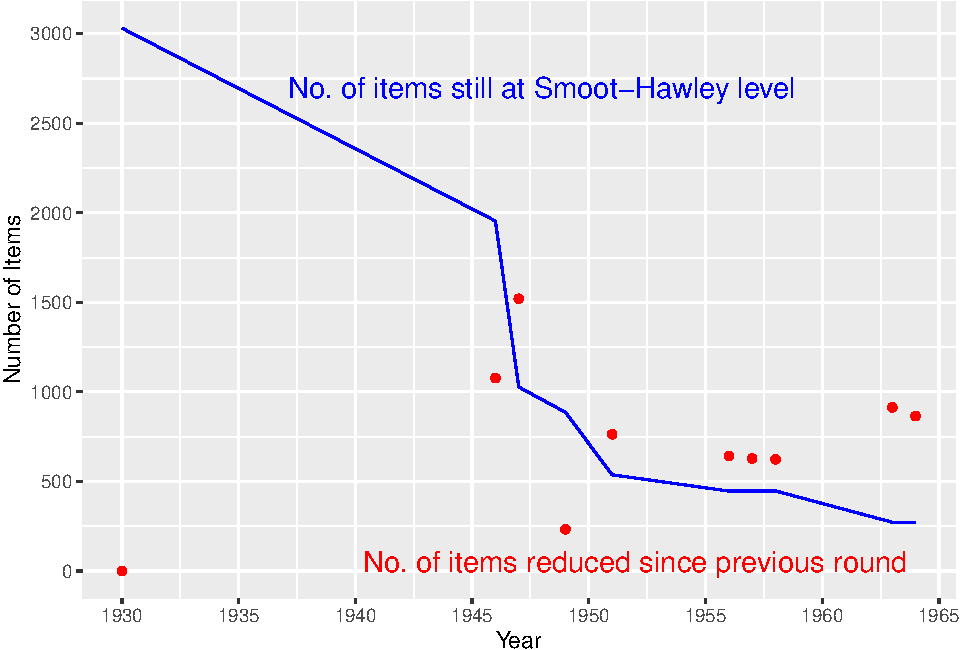
\includegraphics{data-paper_files/figure-latex/ibi-1} \caption{Tariff Reductions by Number of Items}\label{fig:ibi}
\end{figure}

The two related, but distinct measures shown in Figure \ref{fig:ibi} provide a first glimpse into the breadth of negotiations.\footnote{Note that the 1946---just pre-Geneva 1947---embodied bilateral negotiations with nearly twenty countries, the results of which were extended on an MFN basis.} The red dots show how many items saw new commitments in each round. Geneva 1947 saw the largest number of items with commitments of any round: 1520. The Annecy round saw the fewest new commitments at 232; this is in line with expectations since the U.S. only negotiated with new contracting parties in this round.

The blue line connects the dots indicating the number of items that had no negotiated change from Smoot Hawley at each point in our data. For instance, between Smoot Hawley and the start of the Geneva talks in 1946, a little more than one-third of the items in our dataset had some negotiated commitment.\footnote{Note that this does not imply that negotiators made 1000 commitments, as many items were split after 1946.} In the Geneva 1947 round, just under one-third of the items received commitments for the first time. By the end of the Dillon Round phase-in, only 272 items remained with no negotiated commitment.

\hypertarget{from-smoot-hawley-to-dillon-what-was-accomplished}{%
\subsubsection{From Smoot-Hawley to Dillon: what was accomplished?}\label{from-smoot-hawley-to-dillon-what-was-accomplished}}

We find that from the Smoot-Hawley tariffs in 1930 to the last phase in of the Dillon Round in 1964, both specific and \emph{ad valorem} tariffs were cut roughly in half. The mean \emph{ad valorem} tariff binding decreases from 39\% in 1930 to 18.9\% in 1964. The medians are quite close to the means, dropping from 35\% to 15\%. Roughly two-thirds of the items in our dataset have an \emph{ad valorem} tariff.

Things look a bit different for specific tariffs. The mean specific tariff binding decreases from 14 cents in 1930 to 7 cents in 1964, while the median bindings are much smaller, dropping from 0.38 cents to 0.21 cents. Specific tariffs are present for roughly half of the items in our data. Note that summary statistics throughout the paper for specific tariffs are \emph{not} trade weighted; we are in the process of acquiring the trade data required to both trade weight summary statistics and compute \emph{ad valorem} equivalents.

The number of items that have both \emph{ad valorem} and specific components to their tariff in a given round varies from 475 to 505, or a little more than 15\%. Following the categorization in Teti (2000), we refer to these items as \emph{compound}. These items are included in the previous statistics. Also included are \emph{mixed} tariffs, that are specified as having either an \emph{ad valorem} or specific rate, depending on which is higher. Roughly 10\% of our items have some \emph{mixed component}. And about 2\% of the items are \emph{technical} in nature, that is, being defined in non-standard units like the proportion of content that meets some criteria. We do not analyze these categories separately because, insofar as possible, we have integrated them with the basic \emph{ad valorem} and specific types.

\hypertarget{heterogeneity-over-time-round-by-round-liberalization}{%
\subsubsection{Heterogeneity over time: Round-by-Round liberalization}\label{heterogeneity-over-time-round-by-round-liberalization}}

In terms of the time pattern of liberalization, we can confirm a well-known stylized fact: the largest proportional cuts took place between the Smoot-Hawley legislation and the first round of the GATT in Geneva in 1947: average tariffs, both specific and \emph{ad valorem}, fell by about 30\% (see the following two tables).

\begin{table}[!h]

\caption{\label{tab:sp-rd}Decrease in Specific Tariffs by Round}
\centering
\begin{tabular}[t]{lrrrr}
\toprule
  & Mean & \% decrease & Median & \% decrease\\
\midrule
Smoot Hawley & 14.45 & 0.00 & 0.38 & 0.00\\
1946 & 11.56 & 20.03 & 0.38 & 0.00\\
Geneva & 9.12 & 21.10 & 0.31 & 16.67\\
Annecy & 8.96 & 1.71 & 0.28 & 10.00\\
Torquay & 8.06 & 10.08 & 0.24 & 14.93\\
\addlinespace
GenevaA & 7.95 & 1.35 & 0.23 & 2.04\\
GenevaB & 7.85 & 1.30 & 0.22 & 4.00\\
GenevaC & 7.75 & 1.25 & 0.22 & 2.78\\
DillonA & 7.33 & 5.42 & 0.22 & 0.00\\
DillonB & 7.05 & 3.79 & 0.21 & 2.86\\
\bottomrule
\end{tabular}
\end{table}

\begin{table}[!h]

\caption{\label{tab:av-rd}Decrease in Ad Valorem Tariffs by Round}
\centering
\begin{tabular}[t]{lrrrr}
\toprule
  & Mean & \% decrease & Median & \% decrease\\
\midrule
Smoot Hawley & 38.97 & 0.00 & 35.00 & 0.00\\
1946 & 33.95 & 12.88 & 30.00 & 14.29\\
Geneva & 26.46 & 22.07 & 25.00 & 16.67\\
Annecy & 25.56 & 3.40 & 20.00 & 20.00\\
Torquay & 22.14 & 13.38 & 18.75 & 6.25\\
\addlinespace
GenevaA & 21.63 & 2.29 & 17.50 & 6.67\\
GenevaB & 21.36 & 1.24 & 17.50 & 0.00\\
GenevaC & 21.14 & 1.04 & 17.50 & 0.00\\
DillonA & 19.46 & 7.95 & 15.50 & 11.43\\
DillonB & 18.88 & 2.95 & 15.00 & 3.23\\
\bottomrule
\end{tabular}
\end{table}

What will be surprising to many is the the United States was \emph{very} active in negotiating bilateral agreements between 1934 and the start of the GATT negotiations in Geneva in 1947. In terms of \emph{ad valorem} tariffs, a little less than half of the 30\% reduction between Smoot Hawley and Geneva 1947 is directly attributable to the bilateral trade agreements because the U.S. converted all its bilateral concessions into MFN tariffs.\footnote{Only a few pre-existing agreements, such as with Cuba and Philippines, did not have their commitments extended in this way.} Taking into account the 1946 tariff levels, the reduction in \emph{ad valorem} tariffs we find is very close to the figure reported in Irwin (2017 p.~485) of 21\%.

The pattern of reductions after Geneva 1947 is somewhat uneven. From Geneva 1947 to Annecy, the reduction in \emph{ad valorem} tariffs was much smaller at about 3\% for the mean and 20\% for the medians. Reductions in specific tariffs were about half the size of the reductions in \emph{ad valorem} tariffs. Annecy saw small tariff cuts on average in large part because this round was focused on accession: countries like the United States that had joined in Geneva only negotiated with those countries that were newly acceding in the Annecy Round.

In percentage terms, the Torquay Round saw cuts about two-thirds of the size of those in Geneva 1947. Geneva 1956 saw percentage cuts closer to those in Annecy, and for the first time these were phased in. The cuts in tariff averages in the Dillon round were about 5\% for specific tariffs and 10\% for \emph{ad valorem}, while the median for both types of tariffs decreased by about 15\%.

\begin{table}[!h]

\caption{\label{tab:sp-sm-db}Summary Statistics for Specific Tariffs by Round}
\centering
\begin{tabular}[t]{lrrrrrrr}
\toprule
  & Min & 1st Quartile & Mean & Median & 3rd Quartile & Max & N\\
\midrule
Smoot Hawley & 0 & 0.12 & 14.45 & 0.38 & 2.50 & 3000 & 1554\\
1946 & 0 & 0.10 & 11.56 & 0.38 & 2.31 & 1500 & 1541\\
Geneva & 0 & 0.07 & 9.12 & 0.31 & 1.88 & 1000 & 1543\\
Annecy & 0 & 0.07 & 8.96 & 0.28 & 1.75 & 1000 & 1542\\
Torquay & 0 & 0.06 & 8.06 & 0.24 & 1.56 & 750 & 1542\\
\addlinespace
GenevaA & 0 & 0.06 & 7.95 & 0.23 & 1.56 & 750 & 1542\\
GenevaB & 0 & 0.06 & 7.85 & 0.22 & 1.56 & 750 & 1542\\
GenevaC & 0 & 0.06 & 7.75 & 0.22 & 1.56 & 750 & 1539\\
DillonA & 0 & 0.06 & 7.33 & 0.22 & 1.56 & 650 & 1541\\
DillonB & 0 & 0.06 & 7.05 & 0.21 & 1.50 & 550 & 1541\\
\bottomrule
\end{tabular}
\end{table}

\begin{table}[!h]

\caption{\label{tab:av-sm-db}Summary Statistics of Ad Valorem Tariffs by Round}
\centering
\begin{tabular}[t]{lrrrrrrr}
\toprule
  & Min & 1st Quartile & Mean & Median & 3rd Quartile & Max & N\\
\midrule
Smoot Hawley & 5.00 & 25.0 & 38.97 & 35.00 & 50.00 & 105 & 1982\\
1946 & 2.50 & 20.0 & 33.95 & 30.00 & 45.00 & 105 & 1988\\
Geneva & 2.50 & 15.0 & 26.46 & 25.00 & 35.00 & 105 & 1972\\
Annecy & 2.50 & 12.5 & 25.56 & 20.00 & 33.33 & 105 & 1972\\
Torquay & 1.88 & 12.5 & 22.14 & 18.75 & 27.50 & 90 & 1970\\
\addlinespace
GenevaA & 1.88 & 11.5 & 21.63 & 17.50 & 27.50 & 90 & 1970\\
GenevaB & 1.88 & 11.0 & 21.36 & 17.50 & 27.00 & 90 & 1970\\
GenevaC & 1.88 & 10.5 & 21.14 & 17.50 & 25.50 & 90 & 1971\\
DillonA & 1.00 & 10.5 & 19.46 & 15.50 & 25.00 & 90 & 1965\\
DillonB & 0.50 & 10.0 & 18.88 & 15.00 & 25.00 & 90 & 1965\\
\bottomrule
\end{tabular}
\end{table}

\hypertarget{heterogeneity-across-products-schedule-by-schedule-liberalization}{%
\subsubsection{Heterogeneity across products: Schedule-by-Schedule liberalization}\label{heterogeneity-across-products-schedule-by-schedule-liberalization}}

These headline numbers hide variation in magnitude and speed of liberalization across types of products. The data are grouped into 15 industry groups called \emph{schedules} in Smoot Hawley. They range in length from 12 items for Schedule 6 (Tobacco) to 660 items for Schedule 3 (Metals).

\begin{table}[!h]
\centering
\begin{tabular}{cclc}
\toprule
\multicolumn{4}{c}{\bgroup\fontsize{12}{14}\selectfont Schedule Titles\egroup{}} \\
\cmidrule(l{3pt}r{3pt}){1-4}{}
Schedule & Items & Abbreviation & Title\\
\midrule{}
1 & 399 & Chemicals & Chemicals, Oil, and Paints\\
2 & 247 & Glass & Earths, Earthenware, and Glassware\\
3 & 660 & Metals & Metals and Manufactures of\\
4 & 53 & Wood & Wood and Manufactures of\\
5 & 17 & Sugar & Sugar, Molasses, and Manufactures of\\
\addlinespace
6 & 12 & Tobacco & Tobacco and Manufactures of\\
7 & 471 & Ag & Agricultural Products and Provisions\\
8 & 34 & Spirits & Spirits, Wines, and other Beverages\\
9 & 118 & Cotton & Cotton Manufactures\\
10 & 91 & Flax & Flax, Hemp, Jute, and Manufactures of\\
\addlinespace
11 & 161 & Wool & Wool and Manufactures of\\
12 & 38 & Silk & Silk Manufactures\\
13 & 48 & Rayon & Manufactures of Rayon or Other Synthetic Textile\\
14 & 144 & Paper & Papers and Books\\
15 & 538 & Sundries & Sundries\\
\bottomrule{}
\end{tabular}
\end{table}

Note that 98 items switch between \emph{ad valorem} and \emph{specific} at some point. We exclude these items from the analysis in this section because they can distort the summary statistics for small groups.

\begin{table}[!h]

\caption{\label{tab:sp-sc}Reduction in Specific Tariffs by Schedule}
\centering
\begin{tabular}[t]{rrrrrrrrr}
\toprule
Sched & SH\_mean & DB\_mean & mean\_chg & SH\_med & DB\_med & med\_chg & n\_specific & n\\
\midrule
1 & 1.18 & 0.68 & 42.23 & 0.25 & 0.13 & 46.88 & 264 & 396\\
2 & 6.07 & 2.67 & 56.05 & 0.25 & 0.15 & 40.00 & 101 & 232\\
3 & 49.69 & 18.86 & 62.04 & 0.31 & 0.16 & 50.00 & 288 & 620\\
4 & 0.46 & 0.21 & 54.61 & 0.49 & 0.17 & 64.29 & 6 & 53\\
5 & 0.15 & 0.06 & 62.44 & 0.11 & 0.03 & 75.00 & 11 & 17\\
\addlinespace
6 & 9.22 & 3.89 & 57.84 & 3.28 & 1.47 & 55.24 & 12 & 12\\
7 & 11.87 & 3.50 & 70.49 & 0.19 & 0.09 & 50.00 & 355 & 470\\
8 & 2.07 & 0.62 & 70.19 & 0.98 & 0.33 & 66.40 & 33 & 34\\
9 & 0.80 & 0.46 & 42.45 & 0.59 & 0.36 & 39.36 & 8 & 111\\
10 & 0.38 & 0.24 & 36.38 & 0.17 & 0.12 & 31.82 & 42 & 91\\
\addlinespace
11 & 3.15 & 1.96 & 37.82 & 2.50 & 1.94 & 22.50 & 138 & 156\\
12 & NaN & NaN & NaN & NA & NA & NA & 0 & 37\\
13 & 2.50 & 1.45 & 42.06 & 2.81 & 1.56 & 44.44 & 34 & 48\\
14 & 0.85 & 0.49 & 41.57 & 0.31 & 0.12 & 60.00 & 84 & 143\\
15 & 13.64 & 8.25 & 39.52 & 1.56 & 1.00 & 36.00 & 116 & 513\\
\bottomrule
\end{tabular}
\end{table}

Schedule 8 (Spirits, Wines and other Beverages) has all but one of its 34 items covered by a specific tariff and it sees the largest mean tariff in each round. The mean tariff cut is correspondingly largest here, with a decrease of more than 70\% in the average specific tariff from 2\% in Smoot Hawley to 1\% in Dillon.

In contrast, the 11 items with specific tariffs for Schedule 5 (Sugar, Molasses and Manufactures of) start at one of the lowest averages across schedules of 0.2\% but decreases to only 0.1\% by Dillon. The other six items have \emph{ad valorem} tariffs and have the smallest decrease across all schedules for mean \emph{ad valorem} tariffs: from 50.8\% to 31.9\%, which is the largest mean \emph{ad valorem} tariff across all schedules in the Dillon round.

Interestingly, all but one schedule (Schedule 1 -- Chemicals, Oils and Paints) has the mean \emph{ad valorem} tariff decrease by less than the median decrease \emph{ad valorem} tariff, implying a reduction in tariff spikes. For specific tariffs, exactly half of the schedules show this pattern (Schedule 12 -- Silk Manufactures has no specific tariffs).

\begin{itemize}
\item
  Any obvious patterns to which items have largest/smallest cuts?
\item
  Round by round graphs for specific, interesting items
\end{itemize}

\begin{table}[!h]

\caption{\label{tab:sp-sc-rd}Mean Specific Tariffs by Schedule and Round}
\centering
\begin{tabular}[t]{rrrrrrrrrrrrrr}
\toprule
Sched & SH & BG & Ge & An & To & GC & DB & chBG & chGe & chAn & chTo & chGC & chDB\\
\midrule
1 & 1.2 & 1.1 & 1.0 & 1.0 & 0.8 & 0.8 & 0.7 & 8.4 & 9.4 & 0.5 & 18.5 & 4.9 & 9.7\\
2 & 6.1 & 5.5 & 3.9 & 3.1 & 3.0 & 2.8 & 2.7 & 10.0 & 29.0 & 20.7 & 4.0 & 5.4 & 4.6\\
3 & 49.7 & 38.9 & 27.3 & 27.1 & 24.5 & 23.2 & 18.9 & 21.7 & 30.0 & 0.5 & 9.6 & 5.4 & 18.7\\
4 & 0.5 & 0.4 & 0.2 & 0.2 & 0.2 & 0.2 & 0.2 & 17.7 & 47.9 & 0.0 & 0.0 & 0.0 & -5.9\\
5 & 0.2 & 0.1 & 0.1 & 0.1 & 0.1 & 0.1 & 0.1 & 42.9 & 14.8 & 14.5 & 3.2 & 3.1 & 3.8\\
\addlinespace
6 & 9.2 & 7.1 & 5.9 & 5.4 & 4.2 & 3.9 & 3.9 & 22.9 & 16.9 & 8.6 & 22.2 & 6.8 & 0.7\\
7 & 11.9 & 6.9 & 5.2 & 5.2 & 4.1 & 4.1 & 3.5 & 41.9 & 24.6 & 0.2 & 20.6 & 0.4 & 14.7\\
8 & 2.1 & 1.5 & 1.1 & 1.0 & 0.7 & 0.7 & 0.6 & 27.3 & 25.5 & 12.3 & 23.8 & 10.1 & 8.4\\
9 & 0.8 & 0.6 & 0.5 & 0.5 & 0.5 & 0.5 & 0.5 & 19.6 & 18.8 & 0.0 & 10.7 & 0.0 & 1.3\\
10 & 0.4 & 0.3 & 0.3 & 0.2 & 0.2 & 0.2 & 0.2 & 17.3 & 19.2 & 1.3 & 0.2 & 0.2 & 3.2\\
\addlinespace
11 & 3.2 & 2.8 & 2.0 & 2.0 & 2.0 & 2.0 & 2.0 & 9.8 & 28.6 & 0.3 & 2.5 & 0.0 & 0.7\\
12 & NaN & NaN & NaN & NaN & NaN & NaN & NaN & NaN & NaN & NaN & NaN & NaN & NaN\\
13 & 2.5 & 2.4 & 1.7 & 1.6 & 1.5 & 1.5 & 1.4 & 3.7 & 28.8 & 4.3 & 9.5 & 1.8 & 0.6\\
14 & 0.8 & 0.8 & 0.7 & 0.7 & 0.6 & 0.6 & 0.5 & 2.0 & 16.6 & 1.0 & 19.0 & 0.8 & 10.2\\
15 & 13.6 & 12.2 & 10.1 & 10.1 & 9.2 & 8.8 & 8.2 & 10.9 & 16.6 & 0.3 & 9.4 & 3.7 & 6.5\\
\bottomrule
\end{tabular}
\end{table}

\begin{table}[!h]

\caption{\label{tab:av-sc-rd}Mean Ad Valorem by Schedule and Round}
\centering
\begin{tabular}[t]{rrrrrrrrrrrrrr}
\toprule
Sched & SH & BG & Ge & An & To & GC & DB & chBG & chGe & chAn & chTo & chGC & chDB\\
\midrule
1 & 29.9 & 26.2 & 21.0 & 20.6 & 16.9 & 16.1 & 14.1 & 12.2 & 19.8 & 1.9 & 17.9 & 5.2 & 12.1\\
2 & 44.7 & 39.6 & 30.9 & 29.4 & 25.5 & 24.3 & 22.9 & 11.5 & 22.0 & 4.6 & 13.5 & 4.4 & 5.8\\
3 & 37.7 & 32.7 & 26.9 & 25.9 & 21.1 & 19.9 & 17.5 & 13.3 & 17.7 & 3.8 & 18.3 & 5.7 & 12.2\\
4 & 33.9 & 28.7 & 23.2 & 21.5 & 19.9 & 18.3 & 15.1 & 15.4 & 19.2 & 7.4 & 7.4 & 7.7 & 17.7\\
5 & 50.8 & 43.3 & 33.6 & 33.6 & 33.6 & 33.6 & 31.9 & 14.8 & 22.5 & 0.0 & 0.0 & 0.0 & 5.0\\
\addlinespace
6 & 25.0 & 18.8 & 15.6 & 15.6 & 9.4 & 7.8 & 7.8 & 25.0 & 16.7 & 0.0 & 40.0 & 17.3 & 0.0\\
7 & 31.7 & 26.6 & 20.8 & 19.5 & 16.9 & 16.0 & 14.3 & 16.2 & 21.7 & 6.2 & 13.4 & 5.1 & 11.1\\
8 & 60.0 & 60.0 & 60.0 & 60.0 & 30.0 & 30.0 & 30.0 & 0.0 & 0.0 & 0.0 & 50.0 & 0.0 & 0.0\\
9 & 36.6 & 31.4 & 25.4 & 25.0 & 22.9 & 22.7 & 22.3 & 14.3 & 19.0 & 1.6 & 8.4 & 1.0 & 2.0\\
10 & 37.4 & 30.1 & 20.0 & 19.7 & 19.3 & 18.1 & 14.9 & 19.7 & 33.6 & 1.1 & 2.2 & 6.4 & 17.8\\
\addlinespace
11 & 49.2 & 42.7 & 26.3 & 26.1 & 24.6 & 23.9 & 24.9 & 13.2 & 38.3 & 0.7 & 6.0 & 2.9 & -4.5\\
12 & 57.4 & 51.2 & 36.8 & 34.1 & 29.7 & 27.2 & 24.4 & 10.8 & 28.1 & 7.5 & 12.9 & 8.4 & 10.2\\
13 & 52.6 & 49.2 & 35.0 & 33.7 & 28.3 & 26.8 & 26.5 & 6.6 & 28.8 & 3.8 & 15.9 & 5.4 & 1.2\\
14 & 21.7 & 19.2 & 13.3 & 12.5 & 10.9 & 10.2 & 8.7 & 11.3 & 30.9 & 6.1 & 12.5 & 6.6 & 14.7\\
15 & 44.1 & 38.9 & 31.0 & 30.3 & 26.3 & 25.2 & 21.5 & 11.8 & 20.1 & 2.4 & 13.1 & 4.4 & 14.5\\
\bottomrule
\end{tabular}
\end{table}

\hypertarget{notable-findings}{%
\subsection{Notable Findings}\label{notable-findings}}

\hypertarget{importance-of-the-rtaa-in-the-pre-gatt-years}{%
\subsubsection{Importance of the RTAA in the pre-GATT years}\label{importance-of-the-rtaa-in-the-pre-gatt-years}}

Bown and Irwin (2017) present summary data from the USITC on the reduction in rates from Smoot-Hawley to just before Geneva and then to the Geneva rates. We cannot replicate this table until our trade volume and value data are complete.
However, columns ``chBG'' (for change from Smoot Hawley to ``before Geneva'', i.e.~1946) and ``chGe'' (for change from ``before Geneva'' to Geneva (1947) in Tables \ref{tab:sp-sc-rd} and \ref{tab:av-sc-rd} provide the straight item-by-item averages across specific and \emph{ad valorem} tariffs.

However the data is aggregated, it's clear that the bilateral negotiations between 1934 and 1946 made an important contribution to the statutory liberalization of this era. The headline numbers we calculate for mean tariffs in Tables \ref{tab:sp-rd} and \ref{tab:av-rd} are very much in line with the USITC calculations reported by Bown and Irwin (2017) of 21\% pre-Geneva to post-Geneva. We find smaller figures of 20\% and 13\% for the mean reduction in specific and \emph{ad-valorem} tariffs, as compared to the USITC calculation of 33\%, so this is an area where we look forward to finding the effects of trade weighting the data.

\hypertarget{some-items-see-tariff-increases}{%
\subsubsection{Some items see tariff increases}\label{some-items-see-tariff-increases}}

\begin{itemize}
\item
  Para 209, item 6 has tariff double in Geneva56A

  \begin{itemize}
  \tightlist
  \item
    331 item 10 increases specific tariff from 3 to 4 in Torquay
  \item
    911
  \item
    1005.a.3 (something to do with hemp) S-H --\textgreater{} Geneva unchanged; then increase
  \end{itemize}
\end{itemize}

\hypertarget{switching-from-ad-valorem-to-specific-is-rare}{%
\subsubsection{\texorpdfstring{Switching from \emph{ad valorem} to specific is rare}{Switching from ad valorem to specific is rare}}\label{switching-from-ad-valorem-to-specific-is-rare}}

\begin{itemize}
\item
  Metallic magnesium and metallic magnesium scrap, para 375, switches from specific to ad valorem in Geneva56C; reduced from 50 to 45\% in Dillon

  \begin{itemize}
  \item
    1102b (wools nspf) go from ad valorem in every round to specific in Dillon
  \item
    202.a swiches from specific in S-H to ad valorem in Geneva
  \item
    Specific vs.~ad valorem vs.~compound (both specific and ad valorem)
  \item
    Teti (2020) reports that 8\% of U.S. tariffs were specific in 1988-2017
  \item
    Teti (2020) also reports: "Mixed tariffs are expressed as either a specific or an ad valorem rate, depending on which generates the most (or sometimes the least) revenue. Then there are technical tariffs that depend on certain product characteristics for example duties might be 8\% for butter with fat content between 9-40\%. Tariff rate quotas are made up of a low tariff rate on the initial imports (the within-quota quantity) and a very high tariff rate on imports entering above the initial amount (outside-quota quantity).
  \item
    Para 32, ``change of tax formula''? Also 202.a, 232.c,302.d,
  \end{itemize}
\end{itemize}

\hypertarget{analysis}{%
\subsection{Analysis}\label{analysis}}

\begin{itemize}
\item
  What can we say about which / why items have ad valorem vs.~specific?

  \begin{itemize}
  \tightlist
  \item
    Is there variation over time?
  \end{itemize}

  , but we intend to analyze them separately and provide explanation for which items get \emph{ad valorem} protection, which items get specific tariffs, and which get both. We know that the incidence of specific tariffs declines with inflation; this is an important and under-studied aspect of liberalization that we intend to explore.
\item
  Which products `suffer' from large tariff cuts and which products continue to receive protection?
\end{itemize}

\hypertarget{non-u.s.-contracting-parties}{%
\section{Non-U.S. Contracting Parties}\label{non-u.s.-contracting-parties}}

Need table that Matt is creating with number of pages for each schedule for each round

\begin{itemize}
\tightlist
\item
  remember that time series doesn't make sense
\end{itemize}

\hypertarget{conclusion}{%
\section{Conclusion}\label{conclusion}}

Future plans

\begin{itemize}
\item
  What role did the presence of specific tariffs, combined with inflation, have in reducing the total level of tariff protection?

  \begin{itemize}
  \item
    Need trade volume / value / price data
  \item
    include our plans for TOT analysis, what data we're going to use - proof of concept using modern elasticity data would be great, even in a subset of lines
  \end{itemize}
\end{itemize}

\hypertarget{references}{%
\section{References}\label{references}}

Bagwell, K., Staiger, R.W. and Yurukoglu, A. (2020). ``Multilateral trade bargaining: A first look at the GATT bargaining records.'\,' American Economic Journal: Applied Economics, 12, 72-105.

Beshkar, M. and E. W. Bond (2016). ``The Escape Clause in Trade Agreements'\,' in Kyle W. Bagwell and Robert W. Staiger, eds., Handbook of Commerical Policy, Vol. 1B, Amsterdam: 69--106.

Bown, C.P. and M. A. Crowley (2014). ``Emerging Economies, Trade Policy, and Macroeconomic Shocks,'\,' Journal of Development Economics, 111, 261--273.

Bown, C. P. and D. A. Irwin (2017). ``The GATT's Starting Point: Tariff Levels circa 1947,'\,' in Manfred Elsig, Bernard Hoekman, and Joost Pauwelyn (eds.), Assessing the World Trade Organization: Fit for Purpose? Cambridge, UK: Cambridge University Press, 45-74 (Chapter 3).

Broda, C., Limao, N., and D. E. Weinstein (2008). ``Optimal tariffs and market power: The
evidence.'\,' American Economic Review, 98(5), 2032-2065.

Busch, M. L. and K. J. Pelc (2014). ``Law, Politics, and the True Cost of Protectionism: The Choice of Trade Remedies or Binding Overhang,'\,' World Trade Review, 13, 39--64

Chisik, R. (2003). ``Gradualism in free trade agreements: a theoretical justification.'\,' Journal of International Economics, 59, 367-397.

Devereux, M., (1997). ``Growth, specialization, and trade liberalization.'\,' International Economic Review
38, 565-585.

Dobson, J.M. (1976). Two Centuries of Tariffs: The Background and Emergence of the U.S. International Trade Commission. US Government Printing Office.

Evans, J.W. (1971). The Kennedy Round in American Trade Policy: The Twilight of the GATT? Harvard University Press, Cambridge.

Hoda, A. (2018). Tariff Negotiations and Renegotiations under the GATT and the WTO: Procedures and Practices. Cambridge University Press.

Irwin, D. A. (2017). Clashing over commerce: A history of US trade policy. University of Chicago Press.

Krause, L. B. (1962). ``United States Imports, 1947-1958.'\,' Econometrica, 221-238.

Kreinin, M. E. (1967). `\texttt{}Price' vs.~`Tariff' Elasticities In International Trade: A Suggested Reconciliation." The American Economic Review, 57(4), 891-894.

Kuenzel, D. J. (2020). ``WTO tariff commitments and temporary protection: Complements or substitutes?.'\,' European Economic Review, 121, 103-344.

Mavroidis, P. C. (2016). The Regulation of International Trade, Volume 1: GATT (Vol. 1). MIT Press.

Mehlum, H. (1998). ``Why gradualism?'\,' The Journal of International Trade and Economic Development 7, 279-297.

Mussa, M. (1986). ``The adjustment process and the timing of trade liberalization.'\,' In: Choksi, A., Papageorgiou, D. (Eds.), Economic Liberalization in Developing Countries. Basil Blackwell, Oxford.

Rosengarten, G., Summers, J., and and A. Butcher (2017). ``Chapter 7: Tariff Activities'' in \emph{A Centennial History of the United States International Trade Commission}, Benedetto, J., Gamache, L., Holbein, J., and C. Thomsen, eds., USITC Publication 4744, United States International Trade Commission.

Staiger, R. (1995). ``A theory of gradual trade liberalization.'\,' In: Levinsohn, J., Deardorff, A., Stern, R. (Eds.), New Directions in Trade Theory. University of Michigan Press, Ann Arbor, MI, pp.~249-284.

Teti, F. A., (2020). ``30 years of trade policy: Evidence from 5.7 billion tariffs,'\,' ifo Working Paper No.~334.

Zissimos, B, (1997). ``The GATT and gradualism.'\,' The Journal of International Economics, 71, 410-433.

\hypertarget{dataappendix}{%
\section{Data Appendix}\label{dataappendix}}

\hypertarget{sources}{%
\subsection{Data sources}\label{sources}}

\begin{longtable}[]{@{}
  >{\raggedright\arraybackslash}p{(\columnwidth - 4\tabcolsep) * \real{0.33}}
  >{\raggedright\arraybackslash}p{(\columnwidth - 4\tabcolsep) * \real{0.33}}
  >{\raggedright\arraybackslash}p{(\columnwidth - 4\tabcolsep) * \real{0.33}}@{}}
\toprule
File name & Content & Sources \\
\midrule
\endhead
Geneva47\_UNTC & Individual round schedules of Geneva 1947 & UNTC official website, Registration number A-814, Volume number 61. \footnote{\url{https://treaties.un.org/doc/Publication/UNTS/Volume\%2061/v61.pdf}} \\
Annecy\_UNTC & Individual round schedules of Annecy 1949 & UNTC official website, Registration number A-814, Volume number 63. \footnote{\url{https://treaties.un.org/doc/Publication/UNTS/Volume\%2063/v63.pdf}} \\
Torquay\_UNTC & Individual round schedules of Torquay 1951 & UNTC official website, Registration number A-814, Volume number 144. \footnote{\url{https://treaties.un.org/doc/Publication/UNTS/Volume\%20144/v144.pdf}} \\
Geneva56\_UNTC & Individual round schedules of Geneva 1956 & UNTC official website, Registration number A-814, Volume number 245. \footnote{\url{https://treaties.un.org/doc/Publication/UNTS/Volume\%20245/v245.pdf}} \\
Dillon\_UNTC & Individual round schedules of Dillon 1960 & UNTC official website, Registration number A-814, Volume number 440. \footnote{\url{https://treaties.un.org/doc/Publication/UNTS/Volume\%20440/v440.pdf}} \\
Kennedy\_UNTC & Individual round schedules of Kennedy 1964 & UNTC official website, Registration number A-814, Volume number 624. \footnote{\url{https://treaties.un.org/doc/Publication/UNTS/Volume\%20624/v624.pdf}} \\
Tokyo\_UNTC & Individual round schdules of Tokyo 1979 & UNTC official website, Registration number A-814, Volume number 1189. \footnote{\url{https://treaties.un.org/doc/Publication/UNTS/Volume\%201189/v1189.pdf}} \\
Uruguay\_UNTC\_1 & Individual round schedules of Uruguay 1988, till chapter 63 & UNTC official website, Registration number A-814, Volume number 1632. \footnote{\url{https://treaties.un.org/doc/Publication/UNTS/Volume\%201632/v1632.pdf}} \\
Uruguay\_UNTC\_2 & Individual round schedules of Uruguay 1988, rest of the chapters & UNTC official website, Registration number A-814, Volume number 1634. \footnote{\url{https://treaties.un.org/doc/Publication/UNTS/Volume\%201634/v1634.pdf}} \\
Torquay (black white) & Consolidated version of rounds: Geneva47, Annecy and Torquay & The hard copy was borrowed from the Library of University of Texas. We then scanned and digitized the copy. \footnote{\url{https://search.lib.utexas.edu/discovery/fulldisplay?context=L\&vid=01UTAU_INST:SEARCH\&search_scope=MyInst_and_CI\&tab=Everything\&docid=alma991056424989706011}} \\
Tariff Act of 1930 cleaner & Initial tariff schedule of 1930 Smoot-Hawley Tariff Act & Citation information: volume: 46 page: 590 npages: 175 file: STATUTE-46-Pg590.pdf congress: 71 type: publaw number: 361 citation: Pub. Law 71-361 topic: Tariff Act of 1930 title: AN ACT To provide revenue, to regulate commerce with foreign countries, to encourage the industries of the United States, to protect American labor, and for other purposes. June 17, 1930 590 Link for the file \footnote{\url{https://govtrackus.s3.amazonaws.com/legislink/pdf/stat/46/STATUTE-46-Pg590.pdf}}; link for citation information: \footnote{\url{https://github.com/unitedstates/legisworks-historical-statutes/blob/master/data/046.yaml}} \\
US pre-GATT tariff schedule & United States Import Duties, June 1946. & University of Minnesota, Hathitrust Online Library: \footnote{\url{https://catalog.hathitrust.org/Record/100721221?type\%5B\%5D=all\&lookfor\%5B\%5D=united\%20states\%20import\%20duties\%20june\&ft=}} Citation information: United States Tariff Commission. (1946). United States import duties, June 1946. Washington: U.S. Govt. Print. Off. \\
Tariff Classification Study volume 9 & Cross reference schedule between TSUSA system and Smoot-Hawley system in 1962 & The Ohio State University, Hathitrust Online Library: \footnote{\url{https://catalog.hathitrust.org/Record/102256592}} Citation information:United States Tariff Commission. (196061). Tariff classification study. Washington: U.S. Govt. Print. Off.. \\
US 1962 Tariff Act & The first TSUSA tariff schedule system that bridged Dillon round and Kennedy round & The document can be found in various sources, the one we used for digitization is uploaded by University of Illinois at Urbana-Champaign, on Hathitrust Online Library \footnote{\url{https://babel.hathitrust.org/cgi/pt?id=uiug.30112105143967\&view=1up\&seq=3}} \\
\bottomrule
\end{longtable}

\newpage

\hypertarget{examples}{%
\subsection{Examples}\label{examples}}

Here we share images of our source files for an illustrative example. The product displayed is the pharmaceutical chemical \emph{Hexamethylenetetramine}. Under the Smoot Hawley enumeration, it is assigned paragraph number 40, as shown in both the Geneva 1947 tariff schedule and the consolidated file from Torquay. Under the TSUSA system, it is assigned code 425.73.

As the figures below illustrate, the schedules usually consist of three parts: the item number (Smoot Hawley paragraph number or TSUSA code), the product description, and the rate of duty. We structure our data to follow this framework.

\begin{figure}
\centering
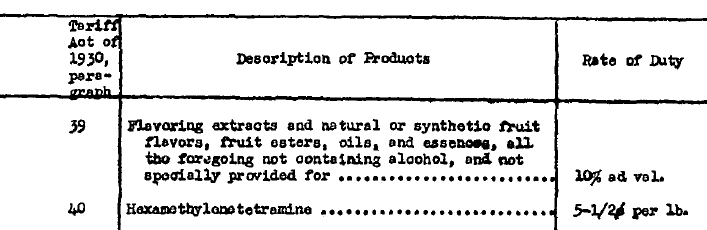
\includegraphics{Geneva47.png}
\caption{Example of an item in Geneva 1947 schedule}
\end{figure}

\begin{figure}
\centering
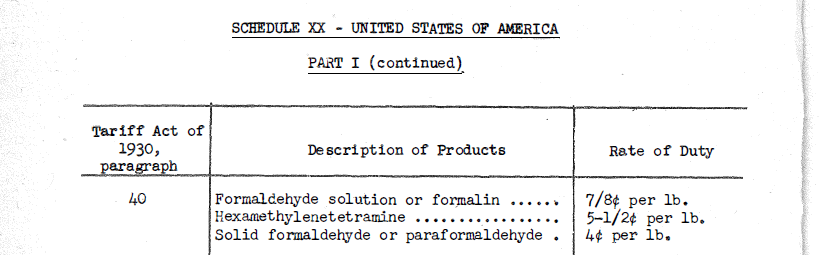
\includegraphics{Torquay.png}
\caption{Example of an item in Torquay\_consolidated schedule}
\end{figure}

\begin{figure}
\centering
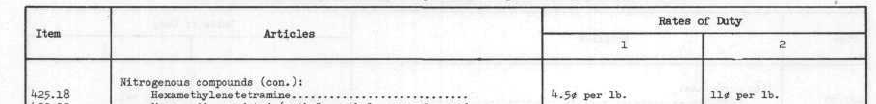
\includegraphics{TSUSA.png}
\caption{Example of an item in 1962 Tariff Act}
\end{figure}

\newpage

\hypertarget{digdetails}{%
\subsection{Details of the Digitization Process}\label{digdetails}}

\hypertarget{the-smoot-hawley-system}{%
\subsubsection{The Smoot-Hawley System}\label{the-smoot-hawley-system}}

We refer to the first document we found---a tariff schedule for the United States that consolidates the concessions in the Geneva, Annecy and Torquay rounds---as ``Torquay (black white).'' This document was in hard copy, borrowed from the University of Texas Libraries. We scanned the hard copy, conducted optical character recognition (OCR) and digitized the file in R. By running the R package \emph{pdftools},\footnote{\url{https://cran.r-project.org/web/packages/pdftools/pdftools.pdf}} we obtain an editable Microsoft Excel file that consists of detailed product descriptions and their corresponding tariff rates. Since ``Torquay (black white)'' contains the schedules of the first three rounds, we were able to construct a benchmark schedule that includes most of the products from Smoot-Hawley through the Dillon Round.

Subsequently, we found more complete and systematic data in the United Nations Treaty Collection (UNTC). Here there are schedules for each round individually. For these we manually entered the United States tariff rate for each round line by line based on the framework we had constructed via ``Torquay (black white).'' To check the reliability of our benchmark file, we compared the three individual rounds we have from the UNTC (i.e., ``Geneva47\_UNTC,'' ``Annecy\_UNTC'' and ``Torquay\_UNTC'') with the consolidated version ``Torquay (black white)'' and found no differences in tariff rates.

Next, we located the original 1930 Tariff Act document (``Tariff Act of 1930 cleaner'') and entered its tariff rates in order to identify the Smoot-Hawley tariffs as a benchmark. The Smoot-Hawley tariffs make sense as a benchmark because they continued to be the prevailing legal tariffs of the U.S. unless modified by subsequent agreement or legislation. We therefore made sure to enter all products in the original Smoot-Hawley into our database. That is, even if some products did not show up in later rounds, they are still included for completeness.

To pin down more precisely the magnitude of the tariff reductions of the first round of GATT negotiations (Geneva 1947), we also digitized the US tariff schedule of the year 1946, using the file ``United State Import Duties June 1946.'' The file contains all tariff changes between 1930 and 1946, both unilaterally and through bilateral negotiations.

With the information above, we are able to identify the magnitude of tariff reductions of every GATT round that uses the Smoot-Hawley tariff system.

After manually cleaning the data in Excel, we save the file as a comma separated values file (csv) in the UTF-8 format and import into R for further data clean, standardizing units for specific tariffs and analysis.

\hypertarget{tsus-system}{%
\subsubsection{TSUS system}\label{tsus-system}}

The TSUS system was first utilized in GATT negotiations in the Kennedy round (1964). To incorporate this new system, we started a separate file for the TSUSA tariffs by digitizing the schedule in the Tariff Act of 1962.\footnote{This act formally changed the tariff system and became effective on August 31, 1963.}

The Tariff Act of 1962 is not related to GATT negotiations. Rather, we digitized it because it provides a comprehensive framework for the TSUS system and helps to fill the gap between the last round under the Smoot-Hawley system (Dillon) and the first round under the TSUS system (Kennedy). Everything we've learned so far indicates that the schedule associated with the Tariff Act 1962 represents the US tariff level after the Dillon round but organized under TSUSA system.\footnote{Two main facts support our belief: (1) we observe that the tariff rates for similar products are exactly the same in the Tariff Act 1962 and the second stage of the Dillon round; (2) the time span between the effective dates of two documents is short: the second stage of Dillon round was effective in 1962 and the Tariff Act of 1962 was effective on August 31, 1963. We will be able to say something more definitive once we have completed the concordance between the Smoot-Hawley and TSUS systems.}

Here we used an approach similar to the one described in the previous subsection. We began with the document ``Tariff Act 1962'' from United States International Trade Commission.\footnote{Several pages are missing in this document, so we also used files from the Hathitrust Digital Library to complete the schedule.} We applied the same optical character recognition tools and constructed the framework of the tariff schedule system in Excel. We then used the tariff schedule files of the Kennedy and Tokyo rounds collected from the UNTC website to manually enter the tariff rate data for each product, line by line. In the Tokyo round, some tariff codes from 1962 and the Kennedy Round are replaced by the introduction of new codes, so we also created an ``exit and entry'' column in our dataset to record these changes. Finally, we followed the same data cleaning and unit-normalization process as in the previous section.

\hypertarget{industrial-classification-systems}{%
\subsection{Industrial Classification Systems}\label{industrial-classification-systems}}

\hypertarget{smoot-hawley-schedule}{%
\subsubsection{Smoot-Hawley: Schedule}\label{smoot-hawley-schedule}}

\begin{longtable}[]{@{}lll@{}}
\toprule
Schedule & Category & Smoot-Hawley Paragraph \\
\midrule
\endhead
1 & Chemicals, Oils, and Paints & 1 to 97 \\
2 & Earths, Earthenware, and Glassware & 201 to 236 \\
3 & Metals and Manufactures of & 301 to 398 \\
4 & Wood and Manufactures of & 401 to 412 \\
5 & Sugar, Molasses, and Manufactures of & 501 to 506 \\
6 & Tobacco and Manufactures of & 601 to 605 \\
7 & Agricultural Products and Provisions & 701 to 783 \\
8 & Spirits, Wines, and Other Beverages & 801 to 815 \\
9 & Cotton Manufactures & 901 to 924 \\
10 & Flax, Hemp, Jute, and Manufactures of & 1001 to 1022 \\
11 & Wool and Manufactures of & 1101 to 1122 \\
12 & Silk Manufactures & 1201 to 1211 \\
13 & Manufactures of Rayon or Other Synthetic Textile & 1301 to 1313 \\
14 & Papers and Books & 1401 to 1413 \\
15 & Sundries & 1501 to 1559 \\
16 & Title II - Free List & 1601 to 1814 \\
\bottomrule
\end{longtable}

\hypertarget{tsusa-section}{%
\subsubsection{TSUSA: Section}\label{tsusa-section}}

\begin{longtable}[]{@{}
  >{\raggedright\arraybackslash}p{(\columnwidth - 4\tabcolsep) * \real{0.11}}
  >{\raggedright\arraybackslash}p{(\columnwidth - 4\tabcolsep) * \real{0.68}}
  >{\raggedright\arraybackslash}p{(\columnwidth - 4\tabcolsep) * \real{0.22}}@{}}
\toprule
Section & Category & TSUSA Code \\
\midrule
\endhead
1 & Animal and Vegetable Products & 100.01 to 193.25 \\
2 & Wood and Paper; Printed Matter & 200.03 to 274.90 \\
3 & Textile Fibers and Textile Products & 300.10 to 390.60 \\
4 & Chemicals and Related Products & 401.02 to 495.20 \\
5 & Nonmetallic Minerals and Products & 511.11 to 548.05 \\
6 & Metals and Metal Products & 601.03 to 696.60 \\
7 & Specified Products: Miscellaneous and Nonemunerated Products & 700.05 to 799.00 \\
8 & Special Classification Provisions & 800 to 870.25 \\
\bottomrule
\end{longtable}

\hypertarget{free-lists}{%
\subsection{Free lists}\label{free-lists}}

Under the Smoot Hawley classification system, items that were free of duty were gathered together into Schedule 16 instead of being integrated into a schedule with like products. That is, the products in Schedule 16 all are free of duty, and unlike the products in Schedules 1-15, the free list products come from many industries. For now, we have not included Schedule 16 in the main data.

Products free-of-duty were organized differently under the TSUSA system. Using both keyword searches and the cross-reference table in Volume 9 of the 1962 Tariff Classification Study, it appears that almost all of the free-of-duty item from Smoot-Hawley are included in the section of TSUSA that corresponds to the industrial characteristics of the product. We will thus integrate the free-of-duty products once we have finished the concordances to the TSUSA Harmonized System classification systems.

Interestingly, the products in the free-of-duty Schedule 16 under the Smoot Hawley classification system entered the tariff schedule gradually. To be more specific, in each round only some of the free-of-duty products from the Tariff Act of 1930 (Smoot Hawley) are included in the tariff schedule.

Between 1930 and when a product enters one of the GATT schedules, the status is not entirely clear. We have not found conclusive evidence to resolve this issue. Given that the Smoot Hawley Act unilaterally set tariff policy free of international commitments, our educated guess is that the U.S. authorities could increase the duty on these products unilaterally. What is clear is that once these products enter a GATT schedule, the U.S. was committed to not subsequently charge a duty on these products. We thus infer that if a product was free of duty in the Tariff Act of 1930 but not included in the free list in the GATT negotiated schedules, the US government either wanted to have more flexibility on this product or had not yet found a negotiating partner who was willing to exchange commitments involving the product.

\hypertarget{int}{%
\subsection{Tariff intervals}\label{int}}

When, in addition to the usual ad valorem or specific tariff, a line also has a minimum or maximum tariff, we classify the line as being of the``tariff interval'' type. For example Paragraph 210 \emph{Rockingham earthenware} in the Geneva 1947 schedule has its rate description as \emph{``20 cents per doz. articles, but not less 7.5\% nor more than 25\%.''}

To incorporate this type of tariff formula, we followed the approach used in the consolidated Torquay schedule and the TSUSA system, that is to divide the single line for that product into multiple lines according to the values of the minimums and maximums. In the consolidated Torquay schedule, \emph{Rockingham earthenware} is listed as three separate lines: \emph{``Rockingham earthenware, valued per dozen articles: under 80 cents - 25\% ad valorem''}, \emph{``Rockingham earthenware, valued per dozen articles: over 80 cents and under 266.67 cents - 20 cents per doz, articles''} and \emph{``Rockingham earthenware, valued per dozen articles: over 266.67 cents - 7.5\% ad valorem''}. Notice that the threshold value for each line is calculated based on the minimum and maximum of tariff rate. With this method, we manually transformed all the tariff interval type lines into separate lines based on their values.

One thing to note is that, as the tariff rates were reduced across rounds, some of the threshold values may also change. Usually these changes are trivial and adding more lines for each newly-calculated threshold would induce more distortion to the data than using the original thresholds. Therefore we use the original threshold value unless the tariff interval formula itself changed over time. We created an ``Intervals'' dummy variable to keep track of lines that are affected by the tariff interval issue.

\hypertarget{split}{%
\subsection{Line splitting}\label{split}}

Another frequent issue in aligning the tariff schedules through time is what we call line splitting. The original product descriptions in the Tariff Act of 1930 paragraphs are often quite general and sometimes ambiguous and we find that the descriptions are often split in later schedules to create product lines whose descriptions are narrower. This seems to happen when the negotiators wanted to apply two different tariffs to what was formerly a single line.

An example of this is Paragraph 24, which is described in the Tariff Act of 1930 as \emph{``Flavoring extracts, and natural or synthetic fruit flavors, fruit esters, oils, and essences, all the foregoing and their combinations.''} In the Dillon round tariff schedule, the paragraph is divided into \emph{``Flavoring extracts, and natural or synthetic fruit flavors, fruit esters, oils, and essences, all the foregoing and their combinations: unfit for beverage purposes, containing of alcohol \ldots{}''} and \emph{``Flavoring extracts, and natural or synthetic fruit flavors, fruit esters, oils, and essences, all the foregoing and their combinations: fit for beverage purposes, containing of alcohol \ldots{}''}.

More restrictions on the descriptions or new types of delineation were introduced as the tariff system evolved. To deal with these splitting lines, we create new lines for each split and enter a uniform tariff rate in earlier schedules for any line that was previously included in the more general (un-split) line. In this way we keep the completeness of the schedule and avoid losing information on differentiated products.

\hypertarget{staging}{%
\subsection{Staging}\label{staging}}

Beginning in the Geneva 1956 round, the tariff reductions were made in multiple stages. In the source documents for Geneva 1956 and Dillon, there is a column for each stage.\footnote{Geneva 1956 has three stages while Dillon has two stages.} Typically there is one year between implementation of each stage. Although most products that are negotiated in each round have different tariffs in each stage, some products do have the tariff rate for more than one stage. To deal with staging, we created separate columns for these stages and track the tariff reduction across stages. However, when comparing the tariff reduction across rounds, we focus on the tariff rate in the final stage.

\hypertarget{gatt-contracting-parties}{%
\subsection{GATT contracting parties}\label{gatt-contracting-parties}}

\textcolor{red}{TO BE ADDED WHEN READY}

\end{document}
